\chapter{Système étudié}
\section{Acétone}
\subsection{Définition et propriétés}
L'acétone est une substance chimique incolore et extrêmement inflammable. Généralement sous forme liquide, il se distingue par une forte odeur suave et un goût piquant.  
L'acétone est totalement miscible dans l'eau et d'autres composants organiques. Ce composant est très volatil avec une tension de vapeur égale à 24.7kPa à 20°C.

Sa température de fusion est de -95,4 °C et celle d'ébullition de 56,53 °C. Elle a une densité relative de 0,819 (à 0 °C).
 
 On peut la trouver naturellement dans les plantes, les arbres, les gaz volcaniques et les feux de forêt, et en tant que sous-produit de la décomposition de la graisse corporelle. Il se trouve aussi dans échappement des véhicules, la fumée de tabac, et les sites d'enfouissement. 
 
L'acétone  est un isomère du propanal et est le composé le plus simple de la famille des cétones. Son nom officiel selon IUPAC est propanone. Elle possède la formule chimique suivante : CH3COCH3

\begin{figure}[h]
\centering
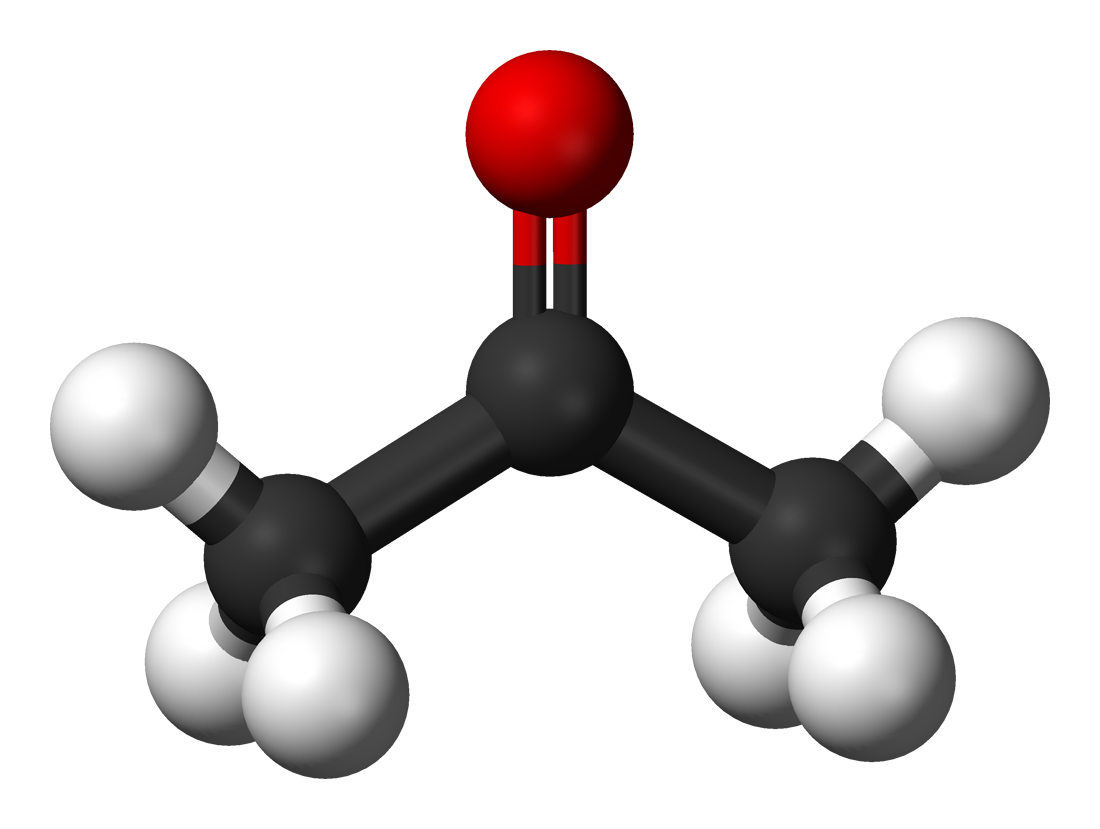
\includegraphics[scale=0.2]{./Figures/Acetone-3D-balls.png}
\caption{Représentation 3D de la molécule Acétone}
\end{figure}

\subsection{Utilisation}
L'acétone est à 75\% pour produire d'autres composants chimique et à 12\% utilisé comme un solvant. Les applications vont de revêtements de surface, des films et d'adhésifs aux produits de nettoyage et les applications pharmaceutique.


D'autres applications grand public et commerciaux comprennent:

\begin{itemize}
\item Les revêtements et les encres
\item Diluants résiniques et les opérations de nettoyage
\item Ciments à usage général
\item Dégraissage et dégommage des agents
\item Peinture, vernis, décapants de vernis
\item Vernis à ongles
\item Divers produits cosmétiques
\end{itemize}

\subsection{Dangers}
L'acétone est de faible toxicité. Il s'agit d'un produit naturel du métabolisme du corps humain.\\
Cependant ce composé peut avoir un impact sur la santé:
\begin{itemize}
\item Irritation des yeux
\item Nocif en cas d'ingestion(pénatration aux poumons)
\item Une exposition prolongé ou répété avec la peau peut causer un assèchement, des gerçures, ou d'irritation.
\item Des concentrations élevées de vapeurs peut provoquer somnolence et irritation des yeux ou des voies respiratoires

\end{itemize}

L'acétone est très inflammable avec une pression de vapeur élevée. Il est de l'utiliser uniquement avec une bonne ventilation et éviter toutes les sources d'inflammation.


\section{N-Hexane}
\subsection{Définition et propriétés}
Hexane est un composé organique constitué d'éléments carbone et de l'hydrogène. Il est produit principalement par l'intermédiaire du raffinage du pétrole.

Les propriétés physiques de l'hexane sont bien connus. Il est le plus couramment trouvé en un liquide incolore. Sa température de fusion d'environ -95,3 ° C et son point d'ébullition est à 67,8 ° C. Il est également une molécule non polaire, ce qui signifie qu'elle n'est pas soluble dans l'eau.

L'hexane est une molécule relativement simple.Il est composé de six atomes de carbone accompagnés par 14 atomes d'hydrogène, ce qui lui donne la formule moléculaire est C6H14. 

\begin{figure}[h]
\centering
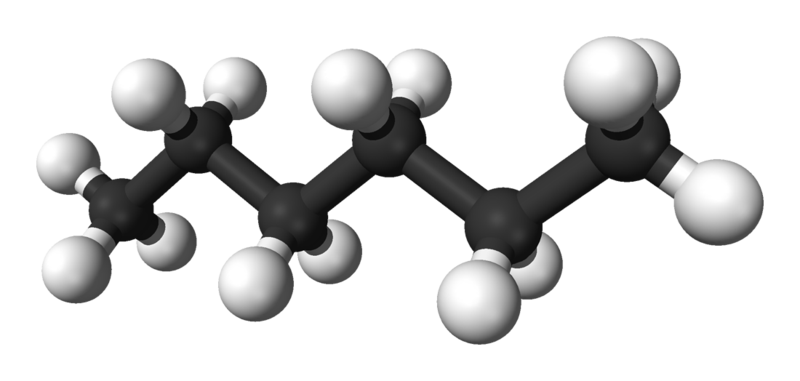
\includegraphics[scale=0.4]{./Figures/Hexane-3D-balls.png}
\caption{Représentation 3D de la molécule Hexane}
\end{figure}

\subsection{Utilisation}


Hexane a de nombreux usages, mais il est surtout connu pour son rôle en tant que solvant. 
Il est utilisé pour extraire les huiles comestibles à partir de graines et de légumes (par exemple, le soja, les arachides, le maïs).

Ces solvants sont utilisés comme agents de nettoyage dans l'imprimerie, textile, meubles, et les industries de fabrication de chaussures.
L'Hexane est aussi utilisé comme un agent de nettoyage et comme dégraissant industriel.
Il peut même être utilisé en tant que liquide dans des thermomètres à basse température. 


\subsection{Dangers}
Une personne est le plus susceptible d'être exposé au n-hexane par inhalation d'air. Comme il est dans l'essence, presque tout le monde est exposé à de très petites quantités de n-hexane dans l'air. L'exposition peut se produire au travail et à la maison et peut avoir des répercussions sur la santé:
\begin{itemize}

\item  Peut causer une irritation légère au niveau des yeux telles que démangeaisons et rougeurs.
\item  Une simple et brève exposition peut provoquer une légère irritation à la peau. Un contact fréquent et prolongé peut causer une irritation plus grave, une délipidation cutanée et une dermatite.
\item L'inhalation Les concentrations élevées de vapeurs sont irritantes pour les voies respiratoires et peuvent causer des maux de tête, étourdissements et  d'autres effets sur le système nerveux, allant même à la  mort. 
\end{itemize}

Une surexposition au n-hexane peut entraîner une détérioration graduelle pouvant être irréversible au système nerveux périphérique, particulièrement aux bras et aux jambes.




